
% !TEX encoding = UTF-8 Unicode 
% !TEX root = FieldGuide.tex

\Sec{Amoroso Distribution}
\label{sec:Amoroso}
\phantomsection\addcontentsline{toc}{subsection}{~~~~~~~~~~~~Amoroso} 
The {\bf Amoroso}  (generalized gamma, Stacy-Mihram) distribution~\cite{Amoroso1925,Johnson1994,Gonzalez2013} is a four parameter,  continuous, univariate, unimodal probability density, with semi-infinite support. The functional form in the most straightforward parameterization is
\begin{align}
\label{Amoroso}  
 \opr{Amoroso}(x&\given  a, \theta, \alpha, \beta) 
\\ \notag&=
\frac{1}{\Gamma(\alpha)} 
\left|\frac{\beta}{\theta}\right|
\left(\frac{x-a}{\theta}\right)^{\alpha \beta -1}
\exp \left\{
-  \left(\frac{x-a}{\theta}\right)^{\beta}
\right\}
\checked
\\ \notag
& \text{for } x,\ a,\ \theta,\ \alpha,\ \beta\  \text{in } \mathbb{R}, 
\ \alpha>0, \ 
\\ \notag
& \text{support } x \geq a \ \text{if}\ \theta > 0,  \ x\leq a  \ \text{if}\  \theta < 0 .
\end{align}

The Amoroso distribution was originally developed to model lifetimes \cite{Amoroso1925}. It occurs as the Weibullization of the standard gamma distribution \eqref{Gamma} and, with integer $\alpha$, in extreme value statistics \eqref{GenFisherTippett}. The Amoroso distribution is itself a limiting form of various more general distributions, most notable the generalized beta \eqref{GenBeta} and generalized beta prime \eqref{GenBetaPrime} distributions~\cite{McDonald1984}.
Many common and interesting probability distributions are special cases or limiting forms of the Amoroso  (See Table~\ref{AmorosoTable}). 


The four real parameters of the Amoroso distribution consist of a location parameter~$a$, 
a scale parameter~$\theta$,  and two shape parameters,~$\alpha$ and~$\beta$. Whenever these symbols appears in special cases or limiting forms, they refer directly to the parameters of the Amoroso distribution.
The shape parameter $\alpha$ is positive, and in many special cases an integer, $\alpha=n$, or half-integer, $\alpha=\tfrac{k}{2}$. The negation of a standard parameter is indicated by a bar, e.g.\ $\bar{\beta} = -\beta$. The chi, chi-squared and related distributions are traditionally parameterized with the scale parameter $\sigma$, where $\theta= (2\sigma^2)^{1/{\beta}}$, and $\sigma$ is the standard deviation of a related normal distribution.  Additional alternative parameters are introduced as necessary. 
  


\begin{table*}[p]
\begin{center}
\label{AmorosoTable}
\caption[Amoroso and gamma distributions -- Special cases]{Special cases of the Amoroso and gamma families}
~\\
{\renewcommand{\arraystretch}{1.1} 
\begin{tabular}{llccccl}
\eqref{Amoroso} &Amoroso & $a$ & $\theta$ & $\alpha$ & $\beta$
\\ \hline
\eqref{Stacy} & Stacy & $0$ & . & . & . \\
\eqref{HalfExpPower} & half exponential power & . & . & $\tfrac{1}{\beta}$ & . \\
\eqref{GenFisherTippett} & gen. Fisher-Tippett  & . & . & $n$ & .  \\
\eqref{FisherTippett} &  Fisher-Tippett & . & . & 1 & .  \\
\eqref{Frechet} &Fr\'{e}chet  & . & . & 1 &  $<\!\!0$  \\
\eqref{GenFrechet} &  generalized Fr\'{e}chet & . & . & $n$ & $<\!\!0$ \\
\eqref{ScaledInvChi} &scaled inverse chi& 0 & . & $\tfrac{1}{2}k$  & -2  \\
\eqref{InvChi} & inverse chi  & 0 & $\frac{1}{\sqrt{2}}$ & $\tfrac{1}{2}k$ & -2 \\
\eqref{InvRayleigh} &  inverse Rayleigh  & $0$ & . & $1$ & -2 \\
\eqref{InvGamma} & inverse gamma & . & . & . & -1 \\
\eqref{ScaledInvChiSqr} & scaled inverse chi-square & 0 & . & $\tfrac{1}{2}k$ & -1 \\
\eqref{InvChiSqr} & inverse chi-square & 0 & $\frac{1}{2}$ & $\tfrac{1}{2}k$ & -1 \\
\eqref{Levy} & L\'{e}vy &  . & . & $\frac{1}{2}$ & -1 \\
\eqref{InvExp} &  inverse exponential & 0  & . & 1 & -1 \\
\eqref{Gamma} &gamma & . & . & . & $1$ \\
\eqref{Gamma} & Erlang & $0$ & $>\!\!0$ & $n$ & $1$ \\
\eqref{StdGamma} &standard gamma & 0 & 1 & . & 1  \\ 
\eqref{PorterThomas} & Porter-Thomas & 0 & 2 & $\tfrac{1}{2}$ & 1 \\
\eqref{ScaledChiSqr} & scaled chi-square & 0 & . & $\tfrac{1}{2}k$ & 1 \\
\eqref{ChiSqr} & chi-square & 0 & 2 & $\tfrac{1}{2}k$ & 1 \\
\eqref{Exp} & exponential & . & . & $1$ & $1$ \\
\eqref{Gamma} & Wien & 0 & . & 4& 1 \\
\eqref{Hohlfeld} & Hohlfeld & 0 & . & $\tfrac{2}{3}$ & $\tfrac{3}{2}$ \\
\eqref{Nakagami} & Nakagami & . & . & . & $2$ \\
\eqref{ScaledChi} &scaled chi& 0 & . & $\tfrac{1}{2}k$  & 2  \\
\eqref{Chi} & chi & 0 & $\sqrt{2}$ & $\tfrac{1}{2}k$ & 2 \\
\eqref{HalfNormal} & half normal & 0 & . & $\tfrac{1}{2}$ & 2 & \\  
\eqref{Rayleigh} & Rayleigh & 0 & . & 1 & 2  \\
\eqref{Maxwell} & Maxwell& 0 & . & $\frac{3}{2}$  & 2  \\
\eqref{WilsonHilferty} &Wilson-Hilferty& 0 & . & .  & 3  \\
\eqref{GenWeibull} & generalized Weibull  & . & . & $n$ & $>\!\!0$  \\
\eqref{Weibull} & Weibull & . & . & 1 &  $>\!\!0$  \\
\eqref{PseudoWeibull} & pseudo-Weibull & . & . & $1$+$\tfrac{1}{\beta}$ &  $>\!\!0$  \\
\\
& $(k,\ n\ \text{positive integers})$
\end{tabular} 
}
\end{center}
\end{table*}



\SSec{Special cases: Miscellaneous}

The gamma distribution ($\beta=1$) and it's special cases are detailed in \secref{sec:Gamma}.

\dist{Stacy} (hyper gamma, generalized Weibull, Nukiyama-Tanasawa, generalized gamma, generalized semi-normal, hydrograph, Leonard hydrograph, transformed gamma)  distribution~\cite{Stacy1962,Dadpay2007}:
\begin{align}
\label{Stacy}
\opr{Stacy}(x \given \theta, \alpha, \beta) 
=& \frac{1}{\Gamma(\alpha)} \left|\frac{\beta}{\theta}\right| \left(\frac{x}{\theta}\right)^{\alpha\beta-1} 
\exp \left\{ -\left(\frac{x}{\theta}\right)^{\beta} \right\} \checked
\\=&  \opr{Amoroso}(x\given  0, \theta, \alpha, \beta) \notag \checked
\end{align}
If we drop the location parameter from $\opr{Amoroso}$, then we obtain the 
Stacy, or generalized gamma distribution, the parent of the gamma family of distributions.
If $\beta$ is negative then the distribution is  {\bf generalized inverse gamma}, the parent of various inverse distributions, including the inverse gamma \eqref{InvGamma} and inverse chi \eqref{InvChi}. 

The Stacy distribution is obtained as the positive even powers,  modulus, and powers of the modulus of a centered, normal random variable \eqref{Normal}, 
\[
\opr{Stacy}\left((2\sigma^2)^{\tfrac{1}{\beta}} ,\tfrac{1}{2}, \beta\right) \sim \Big|\opr{Normal}(0,\sigma)\Big|^{\tfrac{2}{\beta}}
\notag
\checked
\]
and as powers of the sum of squares of $k$ centered, normal random variables. 
\[
\opr{Stacy}\left( (2\sigma^2)^{\tfrac{1}{\beta}} ,\tfrac{1}{2}k, \beta\right) \sim  \left( \sum_{i=1}^{k} \Bigl(\opr{Normal}(0,\sigma)\Bigr)^2\right)^{\tfrac{1}{\beta}}
\notag
\checked
\]



\dist{Pseudo-Weibull} distribution~\cite{Voda1989}:
\begin{align}
\label{PseudoWeibull}
\opr{PseudoWeibull}(x\given a, \theta,\beta)  
=& \frac{1}{\Gamma(1+\tfrac{1}{\beta})} \frac{\beta}{|\theta|} \left(\frac{x-a}{\theta}\right)^{\beta} 
\exp \left\{ -\left(\frac{x-a}{\theta}\right)^{\beta} \right\} \checked
\\ & \text{for } \beta>0 \notag 
\\=&  \opr{Amoroso}(x\given  a, \theta, 1+\tfrac{1}{\beta}, \beta) \notag \checked
\end{align}
Proposed as another model of failure times. 

\dist{Half exponential power} (half Subbotin) distribution~\cite{Gui2013}:
\begin{align}
\label{HalfExpPower}
\opr{HalfExpPower}(x\given a, \theta,\beta)
=& 
\frac{1}{\Gamma(\tfrac{1}{\beta})} 
\left|\frac{\beta}{\theta}\right|
\exp \left\{
-  \left(\frac{x-a}{\theta}\right)^{\beta}
\right\} \checked
\\=&  \opr{Amoroso}(x\given  a, \theta,\tfrac{1}{\beta}, \beta) \notag \checked
\end{align}
As the name implies, half an exponential power \eqref{ExpPower} distribution. Special cases include $\beta=-1$ inverse exponential  \eqref{InvExp}, $\beta=1$ exponential \eqref{Exp}, $\beta=\tfrac{2}{3}$ Hohlfeld  \eqref{Hohlfeld}  and $\beta=2$ half normal \eqref{HalfNormal} distributions. 

\dist{Hohlfeld} distribution~\cite{Hohlfeld2014}:
\begin{align}
\label{Hohlfeld}
\opr{Hohlfeld}(x\given a, \theta)
=& 
\frac{1}{\Gamma(\tfrac{2}{3})} 
\left|\frac{3}{2\theta}\right|
\exp \left\{
-  \left(\frac{x-a}{\theta}\right)^{3/2}
\right\} \checked
\\=&  \opr{HalfExpPower}(x\given a, \theta,\tfrac{3}{2}) \notag \checked
\\=&  \opr{Amoroso}(x\given  a, \theta,\tfrac{2}{3}, \tfrac{3}{2}) \notag \checked
\end{align}
Occurs in the extreme statistics of Brownian ratchets  \cite[Suppl. p.5]{Hohlfeld2014}.





% ========================================================================
\SSec{Special cases: Positive integer \texorpdfstring{$\beta$}{beta}}

\begin{figure}[t]
\begin{center}
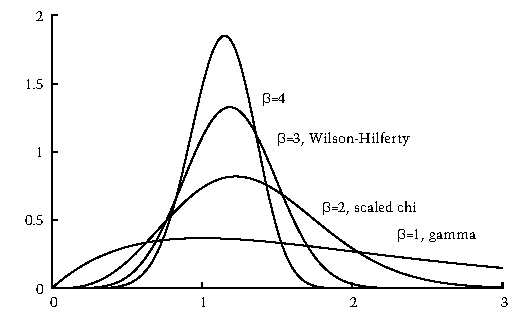
\includegraphics[width=\textwidth]{pdfAmorosoBetaPDF}
\end{center}
\caption[Gamma, scaled chi and Wilson-Hilferty distributions]{Gamma, scaled chi and Wilson-Hilferty distributions, $\opr{Amoroso}(x\given 0,1,2,\beta)$}
\end{figure}

With $\beta=1$ we obtain the gamma family of distributions: gamma \eqref{Gamma}, standard gamma \eqref{StdGamma} and chi square \eqref{ChiSqr} distributions. See \secref{sec:Gamma}.



\dist{Nakagami} (generalized normal, Nakagami-m, m) distribution~\cite{Nakagami1960}:
\begin{align}
\label{Nakagami}
 \opr{Nakagami}&(x \given a , \theta, \alpha) 
\\ \notag 
& =
 \frac{2}{\Gamma(\alpha) |\theta| }
\left(\frac{x-a }{\theta}\right)^{2\alpha -1}
\exp \left\{
-  \left(\frac{x-a }{\theta}\right)^{2}
\right\}
\checked
\\ \notag
& = \opr{Amoroso}(x\given a,\theta, \alpha ,2) \checked
\notag
\end{align}
Used to model attenuation of radio signals that reach a receiver by multiple paths~\cite{Nakagami1960}.




\dist{Half normal} (semi-normal, positive definite normal, one-sided normal) distribution~\cite{Johnson1994}:
%
\begin{align}
\label{HalfNormal}
\opr{HalfNormal}(x \given a, \sigma ) 
&= \frac{2}{\sqrt{2\pi \sigma^2}} 
\exp\left\{-\left( \frac{(x-a)^2}{2\sigma^2}\right) \right\}  
\checked
\\
& \qquad (x-a)/\sigma>0 \notag \\
%&=\opr{ScaledChi}(x \given  \sigma, 1) \notag \checked \\
%&=  \opr{Stacy}(x\given  \sqrt{2\sigma^2} ,\tfrac{1}{2},2) \notag \checked \\
&=  \opr{Amoroso}(x\given  a, \sqrt{2\sigma^2} , \tfrac{1}{2}, 2) \notag  \checked
\end{align}
The modulus of a normal distribution about the mean.

\dist{Chi} ($\chi$) distribution~\cite{Johnson1994}:
%
\begin{align}
\label{Chi}
\opr{Chi}(x \given k) 
&= \frac{ \sqrt{2}}{\Gamma(\tfrac{k}{2})} { \left(\frac{x}{\sqrt{2}}\right)}^{k-1} 
\exp\left\{ -\left( \frac{x^2}{2}    \right)\right\} \checked
\\
& \qquad \text{for positive integer } k \notag \\
& = \opr{ScaledChi}(x\given 1,k) \notag \checked \\
&=  \opr{Stacy}(x\given \sqrt{2}, \sfrac{k}{2}, 2)  \notag \checked \\
&=  \opr{Amoroso}(x\given  0, \sqrt{2} , \sfrac{k}{2}, 2) \notag \checked
\end{align}
The root-mean-square of $k$ independent standard normal variables, or the square root of a chi-square random variable.
\[
\opr{Chi}(k) \sim \sqrt{\opr{ChiSqr}(k)} \checked
\notag
\]

\dist{Scaled chi} (generalized Rayleigh) distribution~\cite{Miller1964,Johnson1994}:
\begin{align}
\opr{ScaledChi}(x \given \sigma, k) 
&= \frac{2}{\Gamma(\tfrac{k}{2}) \sqrt{2\sigma^2}} { \left(\frac{x}{\sqrt{2\sigma^2}}\right)}^{k-1} 
\exp\left\{-\left(\frac{x^2}{2\sigma^2}\right)\right\} 
\notag \checked
\\
& \qquad \text{for positive integer } k \notag \checked \\
&=  \opr{Stacy}(x\given \sqrt{2\sigma^2}, \tfrac{k}{2},2)  \checked
\label{ScaledChi}
\\
&=  \opr{Amoroso}(x \given 0, \sqrt{2\sigma^2}, \tfrac{k}{2}, 2) \checked
\notag 
\end{align}
The root-mean-square of $k$ independent and identically distributed normal variables with zero mean and variance~$\sigma^2$. 


\begin{figure}[t]
\begin{center}
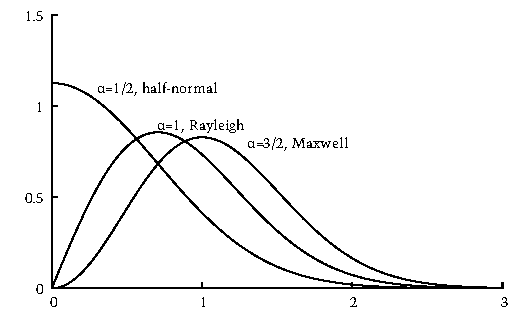
\includegraphics[width=\textwidth]{pdfAmorosoBeta2PDF}
\end{center}
\caption[Half normal, Rayleigh and Maxwell distributions]{Half normal, Rayleigh and Maxwell distributions, $\opr{Amoroso}(x\given 0,1,\alpha,2)$}
\end{figure}



\dist{Rayleigh} (circular normal) distribution~\cite{Strutt1880,Johnson1994}:
%
\begin{align}
\label{Rayleigh}
\opr{Rayleigh}(x \given \sigma) 
&= \frac{1}{\sigma^2 }\ x\  \exp\left\{-\left(\frac{x^2}{2 \sigma^2}\right)\right\}  \checked
\\
&=\opr{ScaledChi}(x \given \sigma, 2) \notag 							\checked \\
&=  \opr{Stacy}(x\given  \sqrt{2\sigma^2} ,1,2) \notag					\checked \\
&=  \opr{Amoroso}(x\given  0, \sqrt{2\sigma^2} , 1, 2) 					\checked \notag 
\end{align}
 The root-mean-square of two independent and identically distributed normal variables with zero mean and variance $\sigma^2$. 
 For instance, wind speeds are approximately Rayleigh distributed, since the horizontal components of the velocity are approximately normal, and the vertical component is typically small~\cite{Justus1978}. 


\dist{Maxwell} (Maxwell-Boltzmann, Maxwell speed, spherical normal) distribution~\cite{Maxwell1860, Abramowitz1965}:
%
\begin{align}
\label{Maxwell}
\opr{Maxwell}(x \given \sigma) 
&= \frac{\sqrt{2}}{\sqrt{\pi} \sigma^3}\ x^2 \exp\left\{-\left(\frac{x^2}{2\sigma^2}\right)\right\}  \checked
 \\
%& x>0,   \notag \\
&=\opr{ScaledChi}(x \given \sigma, 3) \checked \notag \\
&=  \opr{Stacy}(x\given  \sqrt{2\sigma^2} ,\tfrac{3}{2},2) \notag  \checked\\
&=  \opr{Amoroso}(x\given  0, \sqrt{2\sigma^2} , \tfrac{3}{2}, 2) \notag  \checked
\end{align}
The speed distribution of molecules in thermal equilibrium. The root-mean-square of three independent and identically distributed normal variables with zero mean and variance $\sigma^2$.



\dist{Wilson-Hilferty} distribution~\cite{Wilson1931,Johnson1994}:
\begin{align}
\label{WilsonHilferty}
\opr{WilsonHilferty}(x \given \theta, \alpha) 
&= \frac{3}{\Gamma(\alpha)|\theta|} \left(\frac{x}{\theta}\right)^{3 \alpha-1} \exp\left\{-\left(\frac{x}{\theta}\right)^{3}\right\}
\checked
\\ 
&=  \opr{Stacy}(x\given \theta, \alpha, 3) \checked
\notag 
\\ &=  \opr{Amoroso}(x\given  0, \theta, \alpha, 3) \checked
\notag
\end{align}
The cube root of a gamma variable follows the Wilson-Hilferty distribution~\cite{Wilson1931}, which has been used to approximate a normal distribution if $\alpha$ is not too small.
\[
\opr{WilsonHilferty}(x \given \theta, \alpha)  \approx \opr{Normal}(x \given 1-\sfrac{2}{9\alpha},  \sfrac{2}{9\alpha} )
\checked
\notag
\]


A related approximation using quartic roots of gamma variables~\cite{Hawkins1986} leads to   $\opr{Amoroso}(x\given  0, \theta, \alpha, 4)$.


% ====================================================================

\SSec{Special cases: Negative integer \texorpdfstring{$\beta$}{beta}}


With negative $\beta$ we obtain various ``inverse'' distributions related to distributions with positive $\beta$ by the reciprocal transformation $ (\tfrac{x-a}{\theta} ) \mapsto (\tfrac{\theta}{x-a} )$.



\dist{Inverse gamma} (Pearson type V, March, Vinci) distribution~\cite{Pearson1901, Johnson1994}:
\begin{align}
\label{InvGamma}
\opr{InvGamma}(x \given \theta, \alpha) 
&= \frac{1}{\Gamma(\alpha) |\theta|} \left(\frac{\theta}{x-a}\right)^{\alpha+1} 
 \exp\left\{-\left( \frac{\theta}{x-a}   \right)\right\}  \checked
\\
%& = \opr{PearsonV}(x\given a,\theta,\alpha)  \notag \checked \\
&=  \opr{Amoroso}(x\given  a, \theta, \alpha, -1) \notag  \checked
\end{align}
Occurs as the conjugate prior for an exponential distribution's scale parameter~\cite{Johnson1994}, or the prior for variance of a  normal distribution with known mean~\cite{Gelman2004}. Frequently defined with zero scale parameter.


\dist{Inverse exponential} distribution~\cite{Kleiber2003}:
\begin{align}
\label{InvExp}
\opr{InvExp}(x \given a, \theta) 
&= \frac{1}{|\theta|} \left(\frac{\theta}{x-a }\right)^2  \exp\left\{-\left( \frac{\theta}{x-a}   \right)\right\}   \checked \\
&=  \opr{InvGamma}(x\given a,  \theta, 1)  \checked \notag \\
&=  \opr{Amoroso}(x\given  a, \theta, 1, -1) \checked \notag 
\end{align}
Note that the name ``inverse exponential'' is occasionally used for the ordinary exponential distribution \eqref{Exp}.


\begin{figure}[t]
\begin{center}
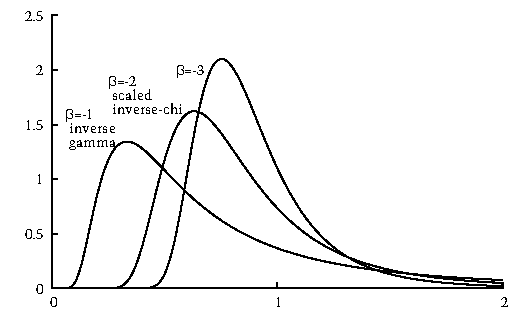
\includegraphics[width=\textwidth]{pdfAmorosoBetaNegPDF}
\end{center}
\caption[Inverse gamma and scaled inverse-chi distributions]{Inverse gamma and scaled inverse-chi distributions, $\opr{Amoroso}(x\given 0,1,2,\beta)$, negative $\beta$.}
\end{figure}




% ===============================
\dist{L\'{e}vy} distribution (van der Waals profile)~\cite{Feller1971}: 
\begin{align}
\label{Levy}
\Levy(x \given a, c) 
&= \sqrt{\frac{|c|}{2\pi}} \frac{1}{(x-a)^{3/2}}  \exp\left\{-\frac{c}{2(x-a)}\right\}  \checked
\\
%&= \opr{PearsonV}(x\given a,\tfrac{c}{2},\tfrac{1}{2})  \checked\notag \\
&=  \opr{Amoroso}(x\given  a, \tfrac{c}{2}, \tfrac{1}{2}, -1) \checked \notag 
\end{align}
The L\'{e}vy distribution is notable for being stable\index{stable distributions}:  a linear combination of identically distributed  L\'{e}vy distributions is again a  L\'{e}vy distribution. The other stable distributions with analytic forms are the normal distribution \eqref{Normal}, which is also a limit of the Amoroso distribution, and the Cauchy distribution \eqref{Cauchy}, which is not. L\'{e}vy distributions describe first passage times in one dimension~\cite{Feller1971}. See also the inverse Gaussian distribution \eqref{InvGaussian}, the  first passage time distribution for Brownian diffusion with drift.
\index{first passage time}
\index{diffusion}


\dist{Scaled inverse chi-square}  distribution~\cite{Gelman2004}:
\begin{align}
\label{ScaledInvChiSqr}
\opr{ScaledInvChiSqr}&(x \given \sigma, k) 
\\ \notag =& \frac{2 \sigma^2}{\Gamma(\tfrac{k}{2}) } \left(\frac{1}{2 \sigma^2x}\right)^{\frac{k}{2}+1} 
\exp\left\{-\left( \frac{1}{2 \sigma^2x}   \right)\right\} \checked
\\
&\qquad  \text{for positive integer } k \notag \\
&=  \opr{InvGamma}(x\given 0, \tfrac{1}{2 \sigma^2}, \tfrac{k}{2}) \notag  \checked \\
%&= \opr{PearsonV}(x\given 0,\tfrac{1}{2 \sigma ^2},\tfrac{k}{2})  \notag  \checked \\
&= \opr{Stacy}(x\given  \tfrac{1}{2 \sigma ^2},\tfrac{k}{2}, -1)  \notag  \checked \\
&=  \opr{Amoroso}(x\given  0, \tfrac{1}{2 \sigma ^2}, \tfrac{k}{2}, -1) \checked \notag 
\end{align}
A special case of the inverse gamma distribution with half-integer $\alpha$. Used as a prior for variance parameters in normal models~\cite{Gelman2004}.




\dist{Inverse chi-square} distribution~\cite{Gelman2004}: 
%
\begin{align}
\label{InvChiSqr}
\opr{InvChiSqr}(x \given k) 
=& \frac{2}{\Gamma(\tfrac{k}{2}) } \left(\frac{1}{2x}\right)^{\frac{k}{2}+1} \exp\left\{-\left( \frac{1}{2x}  \right)\right\}
\checked  \\
&\qquad  \text{for positive integer } k \notag \\
& = \opr{ScaledInvChiSqr}(x\given 1,k)\notag \checked \\
&=  \opr{InvGamma}(x\given 0, \tfrac{1}{2}, \tfrac{k}{2}) \notag \checked \\
%&= \opr{PearsonV}(x\given 0,\tfrac{1}{2},\tfrac{k}{2})  \notag \checked \\
&=  \opr{Stacy}(x\given \tfrac{1}{2}, \tfrac{k}{2},-1) \notag  \checked\\
&=  \opr{Amoroso}(x\given  0, \tfrac{1}{2}, \tfrac{k}{2}, -1)  \checked\notag 
\end{align}
A standard scaled inverse chi-square distribution.



\dist{Scaled inverse chi} distribution~\cite{Lee2012}:
\begin{align}
\label{ScaledInvChi}
 \opr{ScaledInvChi}&(x \given \sigma, k) 
\\ \notag
&= \frac{2 \sqrt{2 \sigma ^2} }{ \Gamma(\tfrac{k}{2})} { \left(\frac{1}{\sqrt{2 \sigma^2} x}\right)}^{k+1} \exp\left\{-\left(\frac{1}{2 \sigma^2 x^2}  \right)\right\} \checked
\\
&=  \opr{Stacy}(x\given \tfrac{1}{\sqrt{2 \sigma^2}}, \tfrac{k}{2}, -2)  \notag \checked \\
&=  \opr{Amoroso}(x\given  0, \tfrac{1}{\sqrt{2 \sigma^2}}, \tfrac{k}{2}, -2) \notag  \checked
\end{align}
Used as a prior for the standard deviation of a normal distribution.

\dist{Inverse chi} distribution~\cite{Lee2012}: 
\begin{align}
\label{InvChi}
\opr{InvChi}(x \given k) 
&= \frac{2\sqrt{2} }{ \Gamma(\tfrac{k}{2})} { \left(\frac{1}{\sqrt{2} x}\right)}^{k+1} \exp\left\{-\left(\frac{1}{2 x^2}  \right)\right\}
\checked
\\
&=  \opr{Stacy}(x\given  \tfrac{1}{\sqrt{2}}, \tfrac{k}{2}, -2)  \notag \checked \\
&=  \opr{Amoroso}(x\given  0, \tfrac{1}{\sqrt{2}} , \tfrac{k}{2}, -2) \notag  \checked
\end{align}


\dist{Inverse Rayleigh} distribution~\cite{Evans2000}:
\begin{align}
\label{InvRayleigh}
\opr{InvRayleigh}(x \given \sigma) 
&= 2 \sqrt{2 \sigma ^2}    \left(\frac{1}{\sqrt{2 \sigma^2} x}\right)^{3} \exp\left\{-\left(\frac{1}{2 \sigma^2 x^2}  \right)\right\}
\checked
\\
&=  \opr{Stacy}(x\given \tfrac{1}{\sqrt{2 \sigma^2}}, 1, -2)  \notag \checked \\
& = \Frechet(x\given 0, \tfrac{1}{\sqrt{2 \sigma^2}}, 2)\notag \\
&=  \opr{Amoroso}(x\given  0, \tfrac{1}{\sqrt{2 \sigma^2}}, 1, -2)  \checked \notag 
\end{align}
The inverse Rayleigh distribution has been used to model  failure time~\cite{Voda1972}.


% ====================================================================



\SSec{Special cases: Extreme order statistics}
\label{SecExtremeOrderStatistic}
\index{extreme order statistics}


\begin{figure}[t]
\begin{center}
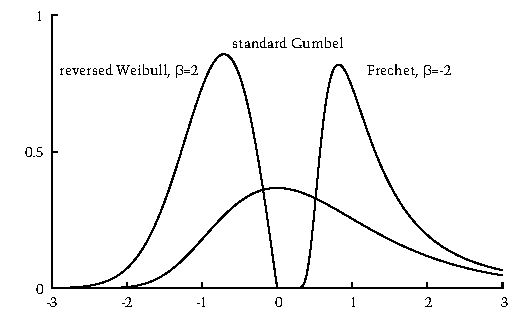
\includegraphics[width=\textwidth]{pdfEVD}
\end{center}
\caption{Extreme value distributions of maxima.}
\end{figure}



\dist{Generalized Fisher-Tippett} distribution~\cite{Smirnov1949,Barndorff-Nielsen1963}:
\begin{align}
\label{GenFisherTippett}  
 \opr{GenFisherTippett}&(x\given  a, \omega, n, \beta) 
\notag
\\ \notag
&=
\frac{n^n}{\Gamma(n)} 
\left|\frac{\beta}{\omega}\right|
\left(\frac{x-a}{\omega}\right)^{n \beta -1}
\exp \left\{
-  n \left(\frac{x-a}{\omega}\right)^{\beta}
\right\} \checked
\\
& \quad \text{for positive integer } n
\\ \notag
& = \opr{Amoroso}(x\given a,{\omega}/{n^{\frac{1}{\beta} }},n,\beta) \checked
\end{align}
If we take $N$ samples from a probability distribution, then asymptotically for large $N$ and $n\ll N$, the distribution of the $n$th largest (or smallest) sample follows a generalized Fisher-Tippett distribution. The parameter $\beta$ depends on the tail behavior of the sampled distribution. Roughly speaking, if the tail is unbounded and decays exponentially then $\beta$ limits to $\infty$, if the tail scales as a power law then $\beta<0$,  and if the tail is finite $\beta>0$~\cite{Gumbel1958}. In these three limits we obtain the Gumbel (\ref{Gumbel}, \ref{GenGumbel}), Fr\'{e}chet (\ref{Frechet}, \ref{GenFrechet}) and Weibull (\ref{Weibull},\ref{GenWeibull}) families of extreme value distribution (Extreme value distributions types I, II and III) respectively. If $\beta/\omega$ is negative we obtain distributions for the $n$th maxima, if positive then the $n$th minima.

% According to wikipedia, McFadden first wrote down unifying form of GEV.

\dist{Fisher-Tippett} (Generalized extreme value, GEV, von Mises-Jenkinson, von Mises extreme value, log-Gumbel, Brody) distribution~\cite{Fisher1928, Mises1936, Gumbel1958,Johnson1995,McFadden1978a}:
\begin{align}
\label{FisherTippett}
\opr{FisherTippett}&(x\given  a , \omega, \beta) 
\\ \notag
&=
\left|\frac{\beta}{\omega}\right|
\left(\frac{x-a}{\omega}\right)^{ \beta -1}
\exp \left\{
-  \left(\frac{x-a}{\omega}\right)^{\beta} 
\right\} \checked
\\ \notag & = \opr{GenFisherTippett}(x\given a, \omega, 1, \beta) \checked
\\ \notag & = \opr{Amoroso}(x\given a, \omega, 1, \beta) \checked
\end{align}
The asymptotic distribution of the extreme value from a large sample. The superclass of type I, II and III (Gumbel, Fr\'{e}chet, Weibull) extreme value distributions~\cite{Mises1936}.  This is the {\bf max stable distribution} (distribution of maxima) with $\beta/\omega<0$ and the {\bf min stable distribution}  (distribution of minima) for $\beta/\omega>0$.


The maximum of two Fisher-Tippett random variables (minimum if $\beta/\omega>0$)  is again a Fisher-Tippett random variable. 
\begin{align*}
\max\Big[ \opr{FisherTippett}(a,\omega_1,\beta),  \opr{FisherTippett}(a, \omega_2,\beta)  \Big]&\\  \sim 
 \opr{FisherTippett}(a, \frac{\omega_1 \omega_2}{(\omega_1^{\beta} + \omega_2^{\beta} )^{1/\beta}},\beta) \checked
\end{align*}
This follows since taking the maximum of two random variables is equivalent to multiplying their cumulative distribution functions, and the Fisher-Tippett cumulative distribution function is $\exp \left\{
-  \left(\frac{x-a}{\omega}\right)^{\beta}
\right\}$.



\dist{Generalized Weibull} distribution~\cite{Smirnov1949,Barndorff-Nielsen1963}:
\begin{align}
\label{GenWeibull}
\opr{GenWeibull}&(x \given a , \omega, n, \beta) 
\\ \notag &=	\frac{n^n}{\Gamma(n)}  \frac{ \beta}{| \omega |} \left(\frac{x-a }{\omega}\right)^{n \beta-1} \exp\left\{-n \left(\frac{x-a }{\omega}\right)^{ \beta}\right\} 
\\ \notag &\quad \text{for } \beta>0 
\\ \notag & = \opr{GenFisherTippett}(x\given a, \omega, n, \beta) \checked
\\ \notag
&= \opr{Amoroso}(x\given  a , {\omega}/{n^{\frac{1}{\beta} }}, n, \beta)  \checked
\end{align}
The limiting distribution of the $n$th smallest value of a large number of  identically distributed random variables that are at least~$a$. 
If $\omega$ is negative we obtain the distribution of the $n$th largest value.




\dist{Weibull}(Fisher-Tippett type III, Gumbel type III, Rosin-Rammler, Rosin-Rammler-Weibull, extreme value type III, Weibull-Gnedenko, stretched exponential) distribution \cite{Weibull1951,Johnson1995}: 
\begin{align}
\label{Weibull}
\opr{Weibull}(x \given a ,\omega, \beta) 
&=	\frac{\beta}{| \omega |} \left(\frac{x-a }{\omega}\right)^{\beta-1} \exp\left\{-\left(\frac{x-a }{\omega}\right)^{\beta}\right\}  \checked
\\ \notag &\quad \text{for } \beta>0 
\\ \notag
& = \opr{FisherTippett}(x\given  a, \omega, \beta) \checked
\\ \notag
&= \opr{Amoroso}(x\given  a , \omega, 1, \beta)  \checked
\end{align}
Weibull\footnote{Pronounced variously as \sl{vay-bull} or \sl{wye-bull}.} is the limiting distribution of the minimum of a large number of  identically distributed random variables that are at least~$a$.  If $\omega$ is negative we obtain a {\bf reversed Weibull} (extreme value type III) distribution for maxima.
Special cases of the Weibull distribution include the exponential ($\beta=1$) and Rayleigh ($\beta=2$)  distributions.
\phantomsection\addcontentsline{toc}{subsection}{~~~~~~~~~~~~Reversed Weibull}

\dist{Generalized Fr\'{e}chet} distribution~\cite{Smirnov1949,Barndorff-Nielsen1963}:
\begin{align}
\label{GenFrechet}
\GenFrechet&(x \given a , \omega, n, \bar{\beta}) 
\\
 \notag 
&=	\frac{n^n}{\Gamma(n)}  \frac{\bar{\beta}}{| \omega |} \left(\frac{x-a }{\omega}\right)^{-n\bar{\beta}-1} 
\exp\left\{-n\left(\frac{x-a }{\omega}\right)^{-\bar{\beta}}\right\} 
\checked
\\ &\quad \text{for } \bar{\beta}>0  \notag
\\ \notag
& = \opr{GenFisherTippett}(x\given a, \omega, n, -\bar{\beta})
\checked
\\ \notag
&= \opr{Amoroso}(x\given  a , {\omega}/{n^{\frac{1}{\beta} }},n,-\bar{\beta}),
\checked
\end{align}
The limiting distribution of the $n$th largest value of a large number identically distributed random variables whose moments are not all finite (i.e. heavy tailed distributions).  (If the shape parameter $\omega$ is negative then minimum rather than maxima.)


\dist{Fr\'{e}chet} (extreme value type II, Fisher-Tippett type II, Gumbel type II, inverse Weibull) distribution~\cite{Frechet1927,Gumbel1958}:
\begin{align}
\label{Frechet}
\Frechet(x \given a , \omega, \bar{\beta}) 
&=	\frac{\bar{\beta}}{| \omega |} \left(\frac{x-a }{\omega}\right)^{-\bar{\beta}-1} 
\exp\left\{-\left(\frac{x-a }{\omega}\right)^{-\bar{\beta}}\right\} \checked
\\ \notag &\quad \text{for } \bar{\beta}>0 \checked
\\  \notag
& = \opr{FisherTippett}(x\given  a, \omega, -\bar{\beta}) \checked
\\ \notag 
&= \opr{Amoroso}(x\given  a , \omega,1,-\bar{\beta})\notag \checked
\end{align}
The limiting distribution of the maximum of a large number identically distributed random variables whose moments are not all finite (i.e. heavy tailed distributions).  (If the shape parameter $\omega$ is negative then minimum rather than maxima.)
Special cases of the Fr\'{e}chet  distribution include the inverse exponential ($\bar{\beta}=1$) and inverse Rayleigh ($\bar{\beta}=2$) distributions.
 





% !TEX encoding = UTF-8 Unicode 
% !TEX root = FieldGuide.tex

\begin{table*}[pt!]

\caption[Amoroso distribution -- Properties]{Properties of the Amoroso distribution}
%\addcontentsline{toc}{subsection}{Amoroso} 

\begin{align*}
\text{\hyperref[PropertiesSec]{Properties}}  \quad& \\
\text{notation} \quad &  \op{Amoroso}(x\given a, \theta, \alpha, \beta)  \checked
\\
\text{PDF} \quad &
\frac{1}{\Gamma(\alpha)} 
\Left|\frac{\beta}{\theta}\Right|
\Left(\frac{x-a}{\theta}\Right)^{\alpha \beta -1}
\exp \Left\{
-  \Left(\frac{x-a}{\theta}\Right)^{\beta}
\Right\}
\checked
\hspace{-8em}
\\ 
\text{CDF / CCDF } \quad  &    1-Q\Left(\alpha, \Left(\tfrac{x - a }{\theta}\Right)^{\beta}\Right) 
\checked & \tfrac{\theta}{\beta}>0 \, \big/ \,  \tfrac{\theta}{\beta}<0
%\\
%& Q(\alpha, \Left(\tfrac{x - a }{\theta}\Right)^{\beta}) 
%& \tfrac{\beta}{\theta}<0
\\
\text{parameters}\quad &   a,\ \theta,\ \alpha,\ \beta\  \text{in } \Real, \ \alpha>0	\checked
\\
\text{support} \quad &     x \geq a &  \theta > 0 \checked
\\
&   x\leq a  &  \theta < 0 	\checked
\\
%\text{median} \quad  &  \cdots
%\\
\text{mode} \quad&   a+ \theta (\alpha-\tfrac{1}{\beta})^{\frac{1}{\beta}}  \checked
& \alpha \beta  \geq 1		\checked
\\ & a & \alpha \beta  \le 1
\\
\text{mean} \quad& a  + \theta \frac{\Gamma(\alpha+\frac{1}{\beta})}{\Gamma(\alpha)}  \checked
& \alpha + \tfrac{1}{\beta} \geq 0
\\
\text{variance}  \quad&   \theta^2 \Left[  \frac{\Gamma(\alpha+\frac{2}{\beta})}{\Gamma(\alpha)}  - 
\frac{\Gamma(\alpha+\frac{1}{\beta})^2}{\Gamma(\alpha)^2}    \Right] \checked
& \alpha + \tfrac{2}{\beta} \geq 0
\\
\text{skew} \quad  &  \Left[  \tfrac{\Gamma(\alpha+\frac{3}{\beta})}{\Gamma(\alpha)} - 3 \tfrac{\Gamma(\alpha+\frac{2}{\beta})\Gamma(\alpha+\frac{1}{\beta})}{\Gamma(\alpha)^2}    + 2  \tfrac{\Gamma(\alpha+\frac{1}{\beta})^3}{\Gamma(\alpha)^3}   \Right]
 \hspace{-3em}
 \\ & \qquad \qquad \qquad \qquad \Big /
 \Left[  \tfrac{\Gamma(\alpha+\frac{2}{\beta})}{\Gamma(\alpha)}  - 
\tfrac{\Gamma(\alpha+\frac{1}{\beta})^2}{\Gamma(\alpha)^2}    \Right]^{3/2}
\hspace{-3em}
\checked
\\
\text{ex. kurtosis} \quad  &  
 \bigg[  \tfrac{\Gamma(\alpha+\frac{4}{\beta})}{\Gamma(\alpha)} 
 - 4 \tfrac{\Gamma(\alpha+\frac{3}{\beta})\Gamma(\alpha+\frac{1}{\beta})}{\Gamma(\alpha)^2}    
 + 6 \tfrac{\Gamma(\alpha+\frac{2}{\beta})\Gamma(\alpha+\frac{1}{\beta})^2}{\Gamma(\alpha)^3}    
\hspace{-3em}
\checked
 \\ & \qquad 
 -3  \tfrac{\Gamma(\alpha+\frac{1}{\beta})^4}{\Gamma(\alpha)^4}   \bigg]
 \Big /
 \Left[  \tfrac{\Gamma(\alpha+\frac{2}{\beta})}{\Gamma(\alpha)}  - 
\tfrac{\Gamma(\alpha+\frac{1}{\beta})^2}{\Gamma(\alpha)^2}    \Right]^{2}
-3 
\hspace{-3em}
\\
\text{entropy} \quad& 
\ln \frac{|\theta| \Gamma(\alpha)}{|\beta|} +\alpha + \Left( \sfrac{1}{\beta} - \alpha\Right) \psi(\alpha) \checked &
\text{\cite{Dadpay2007}}
%\\
%\text{MGF} \quad  &  \cdots
%\\
%\text{CF} \quad  &  \cdots
\end{align*}
\end{table*}




\SSec{Interrelations}

The Amoroso distribution is  a limiting form of  the generalized beta \eqref{GenBeta} and generalized beta prime \eqref{GenBetaPrime} distributions~\cite{McDonald1984}. Limits of the Amoroso distribution include gamma-exponential \eqref{GammaExp}, log-normal \eqref{LogNormal},  and normal \eqref{Normal}~\cite{Johnson1994}  and power function \eqref{PowerFn} distributions. 
\[
\opr{GammaExp}(x\given \nu, \lambda, \alpha) &=  \lim_{\beta\rightarrow\infty} \opr{Amoroso}(x\given \nu+\beta \lambda,-\beta \lambda, \alpha,\beta)
\notag
\checked
\\
 \opr{LogNormal}(x\given a,\vartheta,\sigma) & =
\lim_{\alpha\rightarrow\infty} 
\opr{Amoroso}(x\given  a, \vartheta \alpha^{-\sigma\sqrt{\alpha} } , \alpha, \tfrac{1}{\sigma \sqrt{\alpha}})  
\checked
\notag
\\
\opr{Normal}(x\given \mu,\sigma)   & = 
\lim_{\alpha\rightarrow\infty} \opr{Amoroso}(x\given 0,  \mu- \sigma\sqrt{\alpha}, \tfrac{\sigma}{\sqrt{\alpha}}, \alpha, 1)
\checked
\notag
\]
The log-normal limit is particularly subtle~\cite{Lawless1982}, \secref{sec:Limits}.
\begin{align*} 
\lim_{\alpha\rightarrow\infty} &
\opr{Amoroso}(x\given  a, \vartheta \alpha^{-\sigma\sqrt{\alpha} } , \alpha, \tfrac{1}{\sigma \sqrt{\alpha}})  \checked
\\
& \text{ \sl  Ignore normalization constants and rearrange,}
\\
 \propto & \left(\tfrac{x-a}{\theta}\right)^{-1} \exp\left\{\alpha \ln (\tfrac{x-a}{\theta})^\beta - e^{\ln (\tfrac{x-a}{\theta})^\beta} \right\}
 \checked
\\
& \text{ \sl make the requisite substitutions,}
\\
\propto &
\left(\tfrac{x-a}{\vartheta}\right)^{-1} \exp\left\{\alpha \sfrac{1}{\sigma\sqrt{\alpha}} \ln (\tfrac{x-a}{\vartheta}) - \alpha e^{\sfrac{1}{\sigma\sqrt{\alpha}}  \ln (\sfrac{x-a}{\vartheta})} \right\}
\checked
\\
& \text{ \sl expand second exponential to second order, }
\\
& \text{ \sl (once more ignoring normalization terms) }
\\
 \propto &
\left(\tfrac{x-a}{\vartheta}\right)^{-1} \exp\left\{- \tfrac{1}{2\sigma^2} \left( \ln \tfrac{x-a}{\vartheta} \right)^2 \right\}
\checked
\\
& \text{ \sl and reconstitute the normalization constant.}
\\
= & \opr{LogNormal}(x\given a,\vartheta,\sigma)
\checked
\end{align*}





